%\section{Experiments Setup and Data Sets}
\subsection{Data Collection  and Public Data Sets}
\label{sec:setup}
The usefulness of energy disaggregation algorithms is a function of the aggregated datasets' 
availability. 
Therefore we need to collect this data by installing the corresponding meters and 
sensors and setting up the necessary experiments. 

\subsubsection{Meters}
Generally speaking,
there are two types of data that can be used to disaggregate devices:
AC power and non-AC power information.
To obtain AC power data, real power meter, reactive power meter,
ammeter, voltage meter (usually consolidated into one meter) can be installed to
record different power values, current or voltage values, 
and noises generated by power line.  
Sensors are installed to collect non-AC power data like electromagnetic fields (EMF) 
around devices~\cite{giri_study_2012}, light, and sound~\cite{kim2009viridiscope}.

Figure~\ref{fig_metersConnection} illustrates how
four types of meters/sensors are installed in a building.
After 2-phase power is delivered into the home, %\manishc{usually homes have 2-phase},
three power meters which record real power,
current, and voltage are installed on
these three entry power lines separately.
On each circuit, such as a refrigerator,
a power meter is installed to monitor the
true status of the devices (for validating results).
On the outlet,
a sensor is plugged in to monitor the
voltage noise data.
Besides these AC-power meters,
an electromagnetic field sensor, 
a sound sensor , and a light sensor
may also be installed around devices,
such as refrigerator to capture its electrical magnetic field, 
sound-related, and light-related operations.

\begin{figure}[ht]
\centering
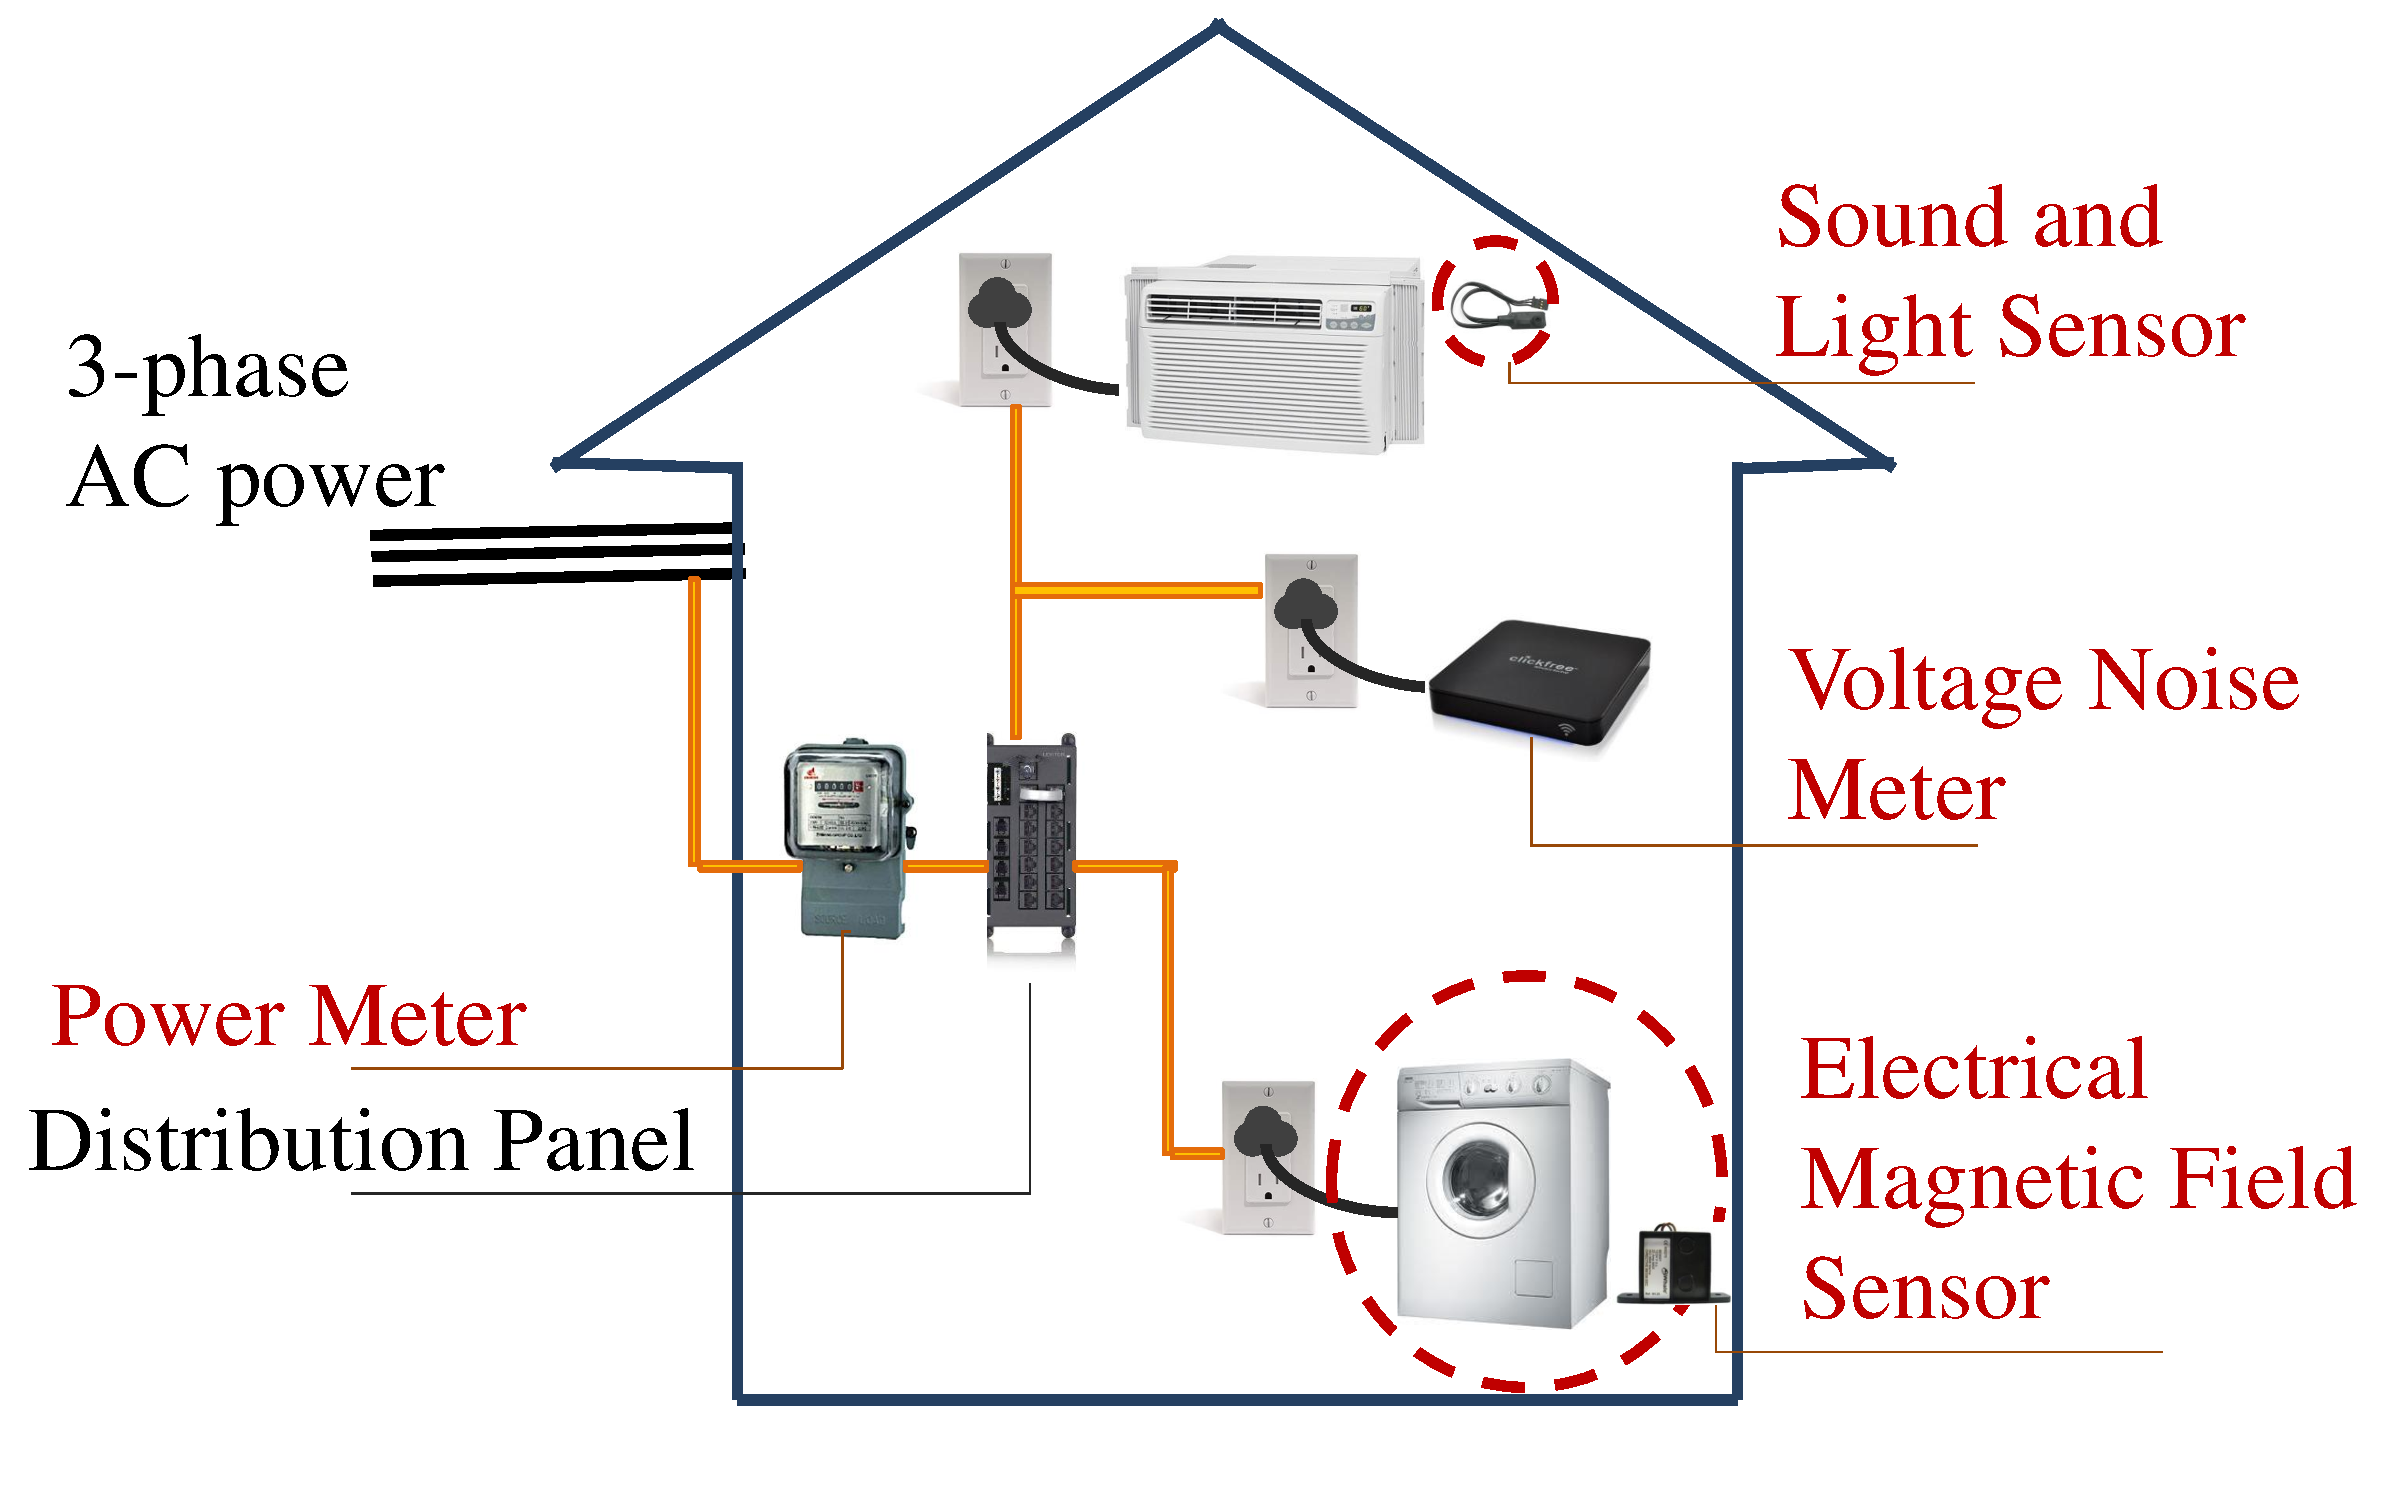
\includegraphics[width=3 in]{figs/metersConnection.pdf}
\caption{Four Types of Meters in a Building.}
\label{fig_metersConnection}
\end{figure}


\begin{table} [h]
\caption{Meters Used in Experiments.}
\label{tab_meters}
\begin{center}
\makebox[\textwidth] {%
\begin{tabular} {|l|l|l|l|}
\hline
Meter Types & Meter Name & Meter Example & Recorded Features \\
\hline
\multirow{4}{*}{AC power} & ammeter & TED, LEM LA55-P~\cite{meterTED} & AC waveform, harmonics \\
\cline{2-4}
& voltage meter & Pico TA041~\cite{meterPico}& voltage waveform, voltage \\
\cline{2-4}
& real power meter & National Instruments USB-9215A~\cite{meterNI} & real power \\
\cline{2-4}
& reactive power meter & TrendPoints EnerSure~\cite{meterTrend}& reactive power \\
\cline{2-4}
& voltage noise meter & Build by author & voltage noise \\
\hline
\multirow{3}{*}{Non-AC power} & electromagnetic field meter & Trifield~\cite{meterEMF}&electromagnetic field \\
\cline{2-4}
& sound sensor& mindstorms~\cite{meterSound}& sound strongness \\
\cline{2-4}
& light sensor & extech~\cite{meterLight}& light strongness \\
\cline{2-4}
& temperature meter & amprobe~\cite{meterTemp}& temperature\\
\hline
\end{tabular}
}
\end{center}
\end{table}


The meters or sensors that have been used in the experiments
are listed in Table~\ref{tab_meters}. 
%\manishc{can you add references for all the 'meter example' in the table} \huijuanc{done.}
Devices like ammeter to gauge the current value, voltage meter to record the voltage,
wattmeter to log the real power, and reactive power meter to record the reactive values 
are easily available.

%Regardless of whether the algorithm uses supervised or unsupervised learning, 
%both the whole-house voltage-current and individual meters for circuit/devices are needed. 
%The circuit level data, that is the ground truth, is necessary for evaluation. 

\subsubsection{Low frequency data and high frequency data}
%Watt meter combines ammeter with voltage meter
%and measures the real power,
%which is the product of root-mean-square(RMS)
%values of voltage and current.
%%\cite{berges2008training} describes how to record these data.
%%%Therefore ,
%%%\begin{equation}
%%%x_{rms}= \sqrt{\frac{1}{T}\int_{0}^{T}x^2(t^{'})dt^{'}}
%%%\end{equation}
%%%here $x(t)$ is the sinusoidal voltage or current as a function of $t$.
%%Also, there is reactive power meter.
%%These meters can be installed on each phase or
%%circuit to monitor the current, voltage values just as Figure\ref{fig_meters}
%%\begin{figure}[ht]
%%\centering
%%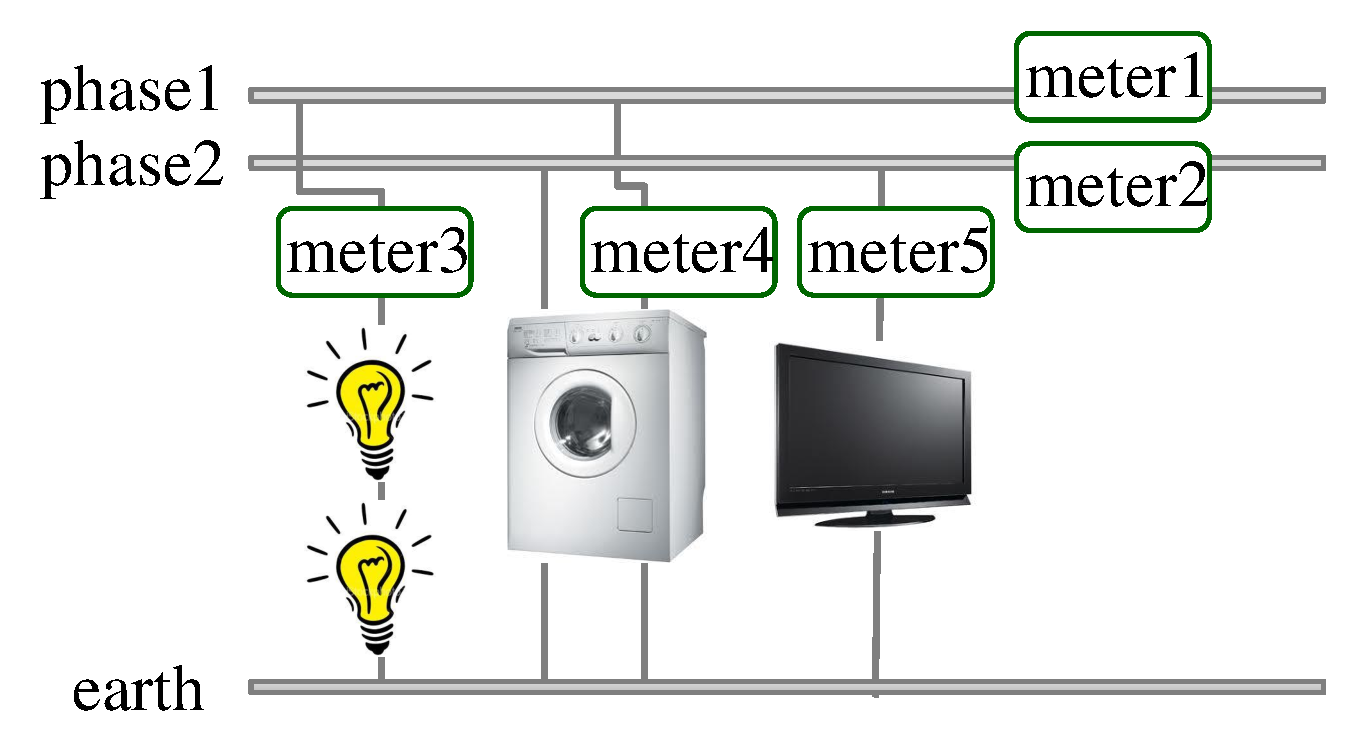
\includegraphics[width=2.5in]{figs/meters.pdf}
%%\caption{Meters on Phases and Circuits}
%%\label{fig_meters}
%%\end{figure}
%For each phase or circuit, meters can be installed
%to record the voltage or current value by voltage
%meter and ammeter.
%Real power is measured by wattmeter.

When meters are installed to monitor the voltage and current,
generally two kinds of data are collected:
low frequency data and high frequency data.

In North America, the basic frequency of voltage or current is
60 Hz. 
If the interval between successive data points is larger than 1/60s, 
the data recorded by the meter is low frequency data, otherwise it is 
high frequency data. 
High frequency data can recover the waveform as
illustrated in Figure~\ref{fig_threephase}.
In practice, only the apparent power
or real power is measured for low frequency data.
For high frequency data, to facilitate the capture of different device characteristics,
normally current and voltage are monitored separately.
In order to capture high order harmonics, the sampling frequency to record the data
should be at least twice as much as the highest frequency.
If targeting to capture harmonics with the highest order $N_{highest}$, 
 the desired harmonics frequency is $N_{highest} \times 60 Hz$,
then the sampling frequency of recorded data $f$ should
meet the criteria that $f \geq N_{highest} \times 1/60 Hz$. 
%\manishc{needs to be fixed} \huijuanc{done.}
%For instance, if the $11th$ harmonics is the highest order 
%we want to use, the recording frequency should be larger than $660$ Hz,
%or $1/660$s.

There are many meters that can record the low frequency power.
However, high frequency data must be monitored by special devices as TED~\cite{meterTED}.
%\manishc{provide ref.}\huijuanc{done.}
Some examples of aggregated energy data collection are mentioned here.
~\cite{berges2010enhancing} install voltage/current meter in a residential
home in Pittsburg, PA.
This experiment chooses 17 on-off devices and installs plug-level meter for
these 17 devices. 
It records the data at a high frequency
(100 kHz). Then features such as real and reactive power, harmonics
are extracted at the frequency of 20 Hz.
Voltage noise data~\cite{patel2007flick} is obtained 
in high frequency sampling rate by
plugging meters into an outlet.~\cite{baranski2003nonintrusive} install an
optical sensor 
%\manishc{what's an optimal sensor?}\huijuanc{optical other than optimal} 
to collect the real power. Then the on-off events are extracted 
from the real power.
A detailed comparison of
whole-house meter, circuit meters and plug-meters 
is given in~\cite{berges2010enhancing}.


%\cite{froehlich2011disaggregated} lists what frequency are needed for
%each kind of features as Figure\ref{fig_setup_froehlich2011disaggregated}.
%http://www.theenergydetective.com/how-does-ted-work
%No matter the voltage or current is recorded
%in high frequency or low frequency,
%the instantaneous values are recorded.
%Therefore the steady states,
%which corresponds to power levels
%conform to Gaussian distribution.
%More concisely, if there's average
%value of a power level $\mu$ and
%$\mu=V_{\mu}$, then
%\begin{displaymath}
%(1-\sqrt2\times V_\mu)\leq \mu \leq (1+\sqrt2)\times V_\mu
%\end{displaymath}
%
%To test whether energy disaggregation succeeds or not,
%proper data needs to be obtained.
%Some datasets are obtained by simulation in experiments.
%But majority of devices are gathered by setting
%experiments.
%Table \ref{tb_setup} lists the devices,
%recorded frequency, extracted features for each paper.

%\begin{figure}[ht]
%\centering
%\includegraphics[width=3 in]{figs/noiseflicker.png}
%\caption{Our prototype system consists of a power line noise analyzer plugged in to an ordinary
%wall outlet and connected to a PC (Courtesy:\cite{patel2007flick}).}
%\label{fig_noiseflicker}
%\end{figure}
%
%\subsubsection{EMI}
%\begin{figure}[ht]
%\centering
%\includegraphics[width=3 in]{figs/installationElectriSense.png}
%\caption{Block diagram of major components of ElectriSense (Courtesy:\cite{gupta2010electrisense}).}
%\label{fig_installationElectriSense}
%\end{figure}

\subsubsection{Public datasets}
Although there are many data sets especially in power industry 
for energy disaggregation, 
majority of them are not open to the public. 
So far there are a few public data sets REDD~\cite{kolter2010redd},
BLUED~\cite{anderson2012blued}, Smart~\cite{barker2012smart}, 
AMPds~\cite{makonin2013ampds}, CASAS~\cite{cook2013CASAS}, iAWE~\cite{batra2013different}, 
and GREEND~\cite{monacchi2014greend}. %(? compare more according to GREEND papers)
The first open data set REDD, when introduced, opened the doors for several 
researchers to attack the energy disaggregation problem.

So far, a majority of the data is stored as plain text. 
Some work proposes to store these datasets in database~\cite{lai2012database}  
or builds a metadata as a standard~\cite{kelly2014metadata}. 

